\section{Difa Al Fansha}
\subsection{Teori}

\begin{enumerate}

	\item Klasifikasi Biner
		Klasifikasi biner adalah mepresentasikan suatu hal kedalam bilangan biner, lalu mengelompokkannya.
		
			\begin{figure}[H]
				\begin{center}
				 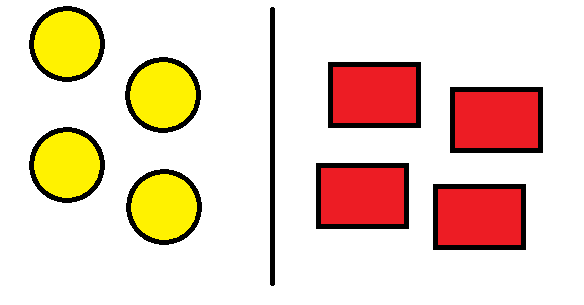
\includegraphics[width=10cm]{figures/1174076/figures2/1.png}
				 \caption{Biner}	
				\end{center}
			\end{figure}
		
	\item Definisi Supervised Learning, Klasifikasi, Regresi, Unsupervised Learning, Data Set, Training Set dan Testing Set
		
		\begin{itemize}
			\item Supervised Learning
				\paragraph{}
				Supervised learning adalah sebuah pendekatan yang sudah ada datanya dan tinggal mengelompokkan data barus tersebut pada data yang sudah ada.\\
				
				Contoh :\\
				Saya punya banyak buku dan saya kategorikan sebagi berikut Komik, Novel, dan Akademik.
				Kemudian saya membeli sebuah komik one piece, tentu saja saya meletakkannya di bagian komik.
	
			\begin{figure}[H]
				\begin{center}
				 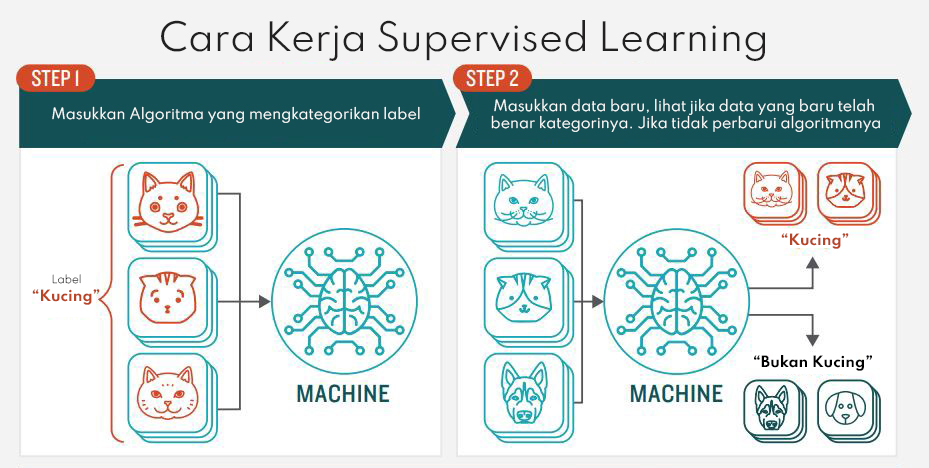
\includegraphics[width=10cm]{figures/1174076/figures2/2.jpg}
				 \caption{Supervised}	
				\end{center}
			\end{figure}
				
				
			\item Unsupervised Learning
				\paragraph{}
				Unsupervised learning tidak memiliki data, sehingga kita mengelompokkan data tersebut menjadi beberapa bagian.\\
				Contoh :\\
				Saya membeli banyak komik, lalu saya mengelompokkannya sesuai dengan kriteria Manga, Manhwa dan Manhua.

			\begin{figure}[H]
				\begin{center}
				 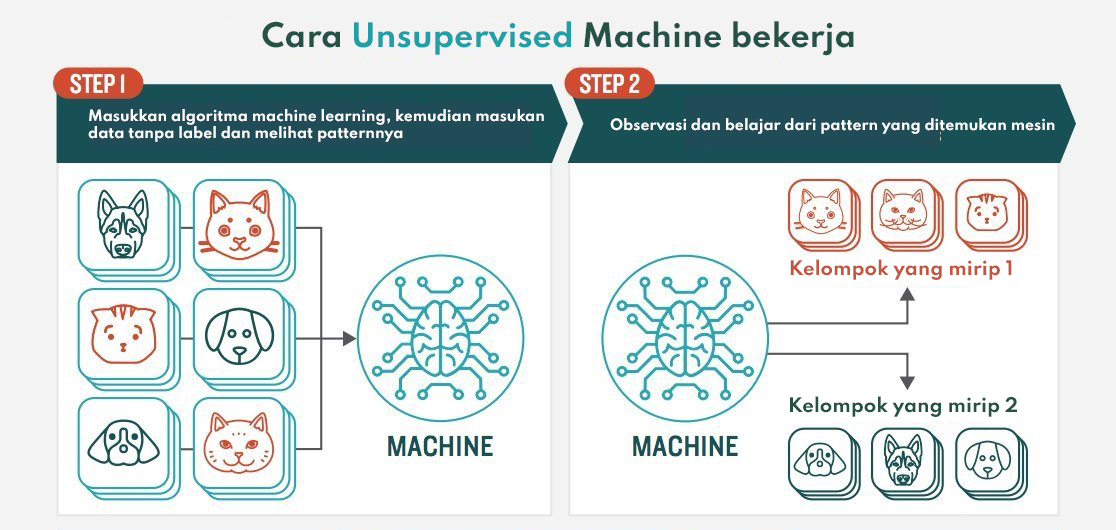
\includegraphics[width=10cm]{figures/1174076/figures2/3.jpg}
				 \caption{Unsupervised}	
				\end{center}
			\end{figure}
				
			\item Clustering
				\paragraph{}
				Mengelompokkan data yang memiliki kesamaan.\\
				Contoh :\\
				Saya mengelompokkan one piece dan hunter x hunter karena keduanya memiliki Genre adventure.

			\begin{figure}[H]
				\begin{center}
				 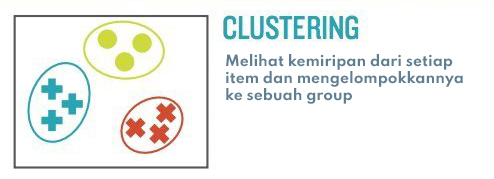
\includegraphics[width=10cm]{figures/1174076/figures2/4.jpg}
				 \caption{Clustering}	
				\end{center}
			\end{figure}	
		
		\end{itemize}	
		
	\item Evaluasi dan Akurasi
		\begin{itemize}
		\item Evaluasi adalah tentang bagaimana kita dapat mengevaluasi seberapa baik model bekerja dengan mengukur akurasinya. 
		
		\item Dan akurasi akan didefinisikan sebagai persentase kasus yang diklasifikasikan dengan benar. 

		\end{itemize}
		
	\item Cara membuat dan membaca confusion matrix : 
	
	\begin{itemize}
		\item Tentukan pokok permasalahan dan atributanya, misal gaji dan listik.
		\item Buat pohon keputusan
		\item Lalu data testingnya
		\item Lalu mencari nilai a, b, c, dan d. Semisal a = 5, b = 1, c = 1, dan d = 3. 
		\item Selanjutnya mencari nilai recall, precision, accuracy, serta dan error rate.
	\end{itemize}
	
	paragraph{}
	Berikut adalah contoh dari confusion matrix :\\
	\begin{itemize}
		\item Recall =3/(1+3) = 0,75
		\item Precision = 3/(1+3) = 0,75 
		\item Accuracy =(5+3)/(5+1+1+3) = 0,8 
		\item Error Rate =(1+1)/(5+1+1+3) = 0,2
	\end{itemize}
	
	\item Bagaimana K-fold cross validation bekerja.
	\begin{itemize}
		\item Total instance dibagi menjadi N bagian.
		\item Fold yang pertama adalah bagian pertama menjadi data uji (testing data) dan sisanya menjadi training data.
		\item Lalu hitung akurasi berdasarkan porsi data tersebut dengan menggunakan persamaan.
		\item Fold yang kedua adalah bagian kedua, yang menjadi data uji(testing data)dan sisanya training  data.
		\item Kemudian hitung akurasi berdasarkan porsi data tersebut.
		\item Dan seterusnya hingga habis mencapai fold ke-K.
		\item Terakhir hitung rata-rata akurasi K buah.
	\end{itemize}
	
	\begin{figure}[H]
		\begin{center}
		 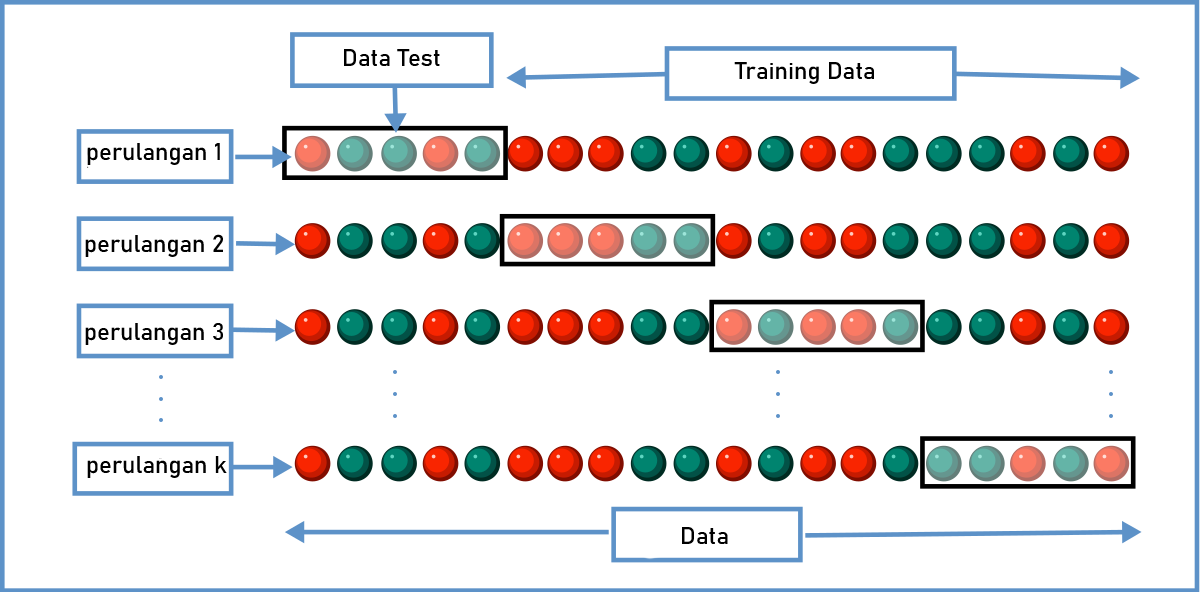
\includegraphics[width=10cm]{figures/1174076/figures2/7.png}
		 \caption{Contoh K-Fold Cross Validation}	
		\end{center}
	\end{figure}		
			

	\item Apa itu Decision Tree
	Decision tree adalah model prediksi menggunakan struktur pohon atau struktur berhirarki
Konsep dari pohon keputusan adalah mengubah data menjadi decision tree dan aturan-aturan keputusan. 
Manfaat utama dari penggunaan decision tree adalah kemampuannya untuk mem-break down proses pengambilan keputusan yang kompleks menjadi lebih simple, sehingga pengambil keputusan akan lebih menginterpretasikan solusi dari permasalahan.

	
	\begin{figure}[H]
		\begin{center}
		 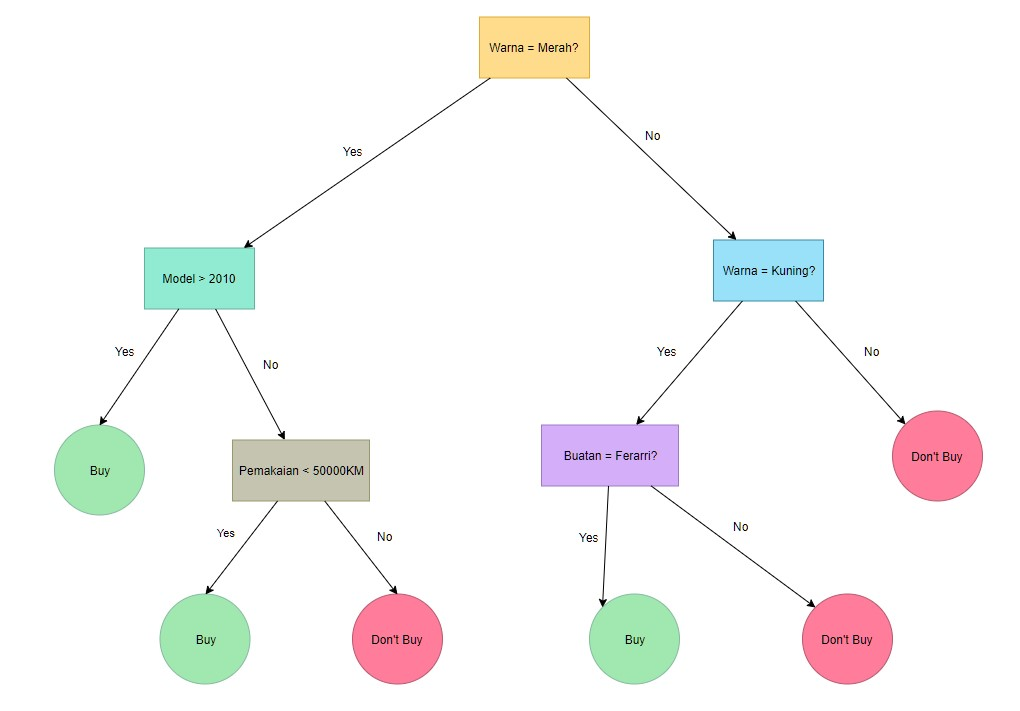
\includegraphics[width=10cm]{figures/1174076/figures2/8.jpg}
		 \caption{Decision Tree}	
		\end{center}
	\end{figure}
	
	
	\item Information Gain
	Information gain didasarkan pada penurunan entropi setelah data set dibagi pada atribut. 
Membangun decision tree adalah semua tentang menemukan atribut yang mengembalikan perolehan informasi tertinggi (mis: Cabang yang paling homogen).
	
	\begin{figure}[H]
		\begin{center}
		 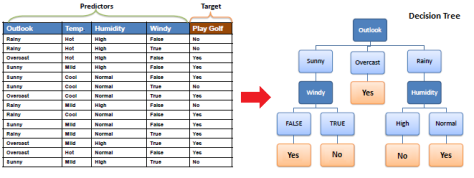
\includegraphics[width=10cm]{figures/1174076/figures2/9.png}
		 \caption{Information Gain}	
		\end{center}
	\end{figure}
\end{enumerate}

\subsection{Praktek}
	\begin{enumerate}
		\item soal 1
			\lstinputlisting[firstline=7, lastline=13]{src/1174076/src2/Student_performance.py}
		\item soal 2
			\lstinputlisting[firstline=14, lastline=19]{src/1174076/src2/Student_performance.py}
		\item soal 3
			\lstinputlisting[firstline=21, lastline=28]{src/1174076/src2/Student_performance.py}
		\item soal 4
			\lstinputlisting[firstline=29, lastline=51]{src/1174076/src2/Student_performance.py}

		\item soal 5
			\lstinputlisting[firstline=52, lastline=62]{src/1174076/src2/Student_performance.py}
		\item soal 6
			\lstinputlisting[firstline=63, lastline=74]{src/1174076/src2/Student_performance.py}
		\item soal 7
			\lstinputlisting[firstline=75, lastline=82]{src/1174076/src2/Student_performance.py}
		\item soal 8
			\lstinputlisting[firstline=83, lastline=86]{src/1174076/src2/Student_performance.py}
		\item soal 9
			\lstinputlisting[firstline=87, lastline=95]{src/1174076/src2/Student_performance.py}
		\item soal 10
			\lstinputlisting[firstline=96, lastline=102]{src/1174076/src2/Student_performance.py}
		\item soal 11
			\lstinputlisting[firstline=103, lastline=116]{src/1174076/src2/Student_performance.py}
		\item soal 12
			\lstinputlisting[firstline=117, lastline=122]{src/1174076/src2/Student_performance.py}
		

		
	\end{enumerate}
	
\subsection{Bukti tidak plagiat}

\subsection{Link Youtube}
https://www.youtube.com/watch?v=z3HrIeo2N\_c
	